\documentclass{classrep}
\usepackage[utf8]{inputenc}
\usepackage{color}
\usepackage{graphicx}
\usepackage{float}
\graphicspath{ {./images/} }

\studycycle{Informatyka, studia dzienne, I st.}
\coursesemester{VI}

\coursename{Komputerowe systemy rozpoznawania}
\courseyear{2019/2020}

\courseteacher{Marcin Kacprowicz}
\coursegroup{wtorek, 14:00}

\author{
  \studentinfo{Sebastian Kaźmierski}{216795} \and
  \studentinfo{Bartosz Paluszkiewicz}{216856} 
}

\title{Zadanie 1: Ekstrakcja cech, miary podobieństwa, klasyfikacja}


\begin{document}
\maketitle

\section{Cel}
{
Celem zadania jest stworzenie aplikacji która wykorzystując metodę Knn będzie wykonywała klasyfikację artykułów w dwóch kategoriach (Places,Topics). Aplikacja ma również implementować moduł ekstrakcji cech który będzie obliczał wartości cech klasyfikowanych artykułów. Po stworzeniu aplikacji przy jej wykorzystaniu zostaną przeprowadzone eksperymenty z różnymi wartościami parametrów metody Knn.}

\section{Wprowadzenie}
\subsection{Klasyfikator}
Zaimplementowany klasyfikator zbioru tekstów wykorzystuje algorytm k najbliższych sąsiadów (k-nn, k nearest keighbours), który jest jednym z bezparametrowych metod klasyfikacji statystycznej.\newline
W trakcie działania nie tworzy wewnętrznej reprezentacji danych uczących, lecz przechowuje wszystkie wzore uczące i dopiero w momencie pojawienia się wzorca testującego szuka rozwiązania, wyznaczając odległość do wszystkich wzorców.\newline
Bezparametrowość algorytmu objawia się brakiem założeń co do rozkładu podstawowych danych, np. rozkładu jednostajnego.\newline\newline

\subsection{Wektor cech}
Do ekstrakcji danych wykorzystaliśmy wektor następujących cech:
\begin{enumerate}
  \item Liczba wszystkich słów kluczowych w pierwszych 10\% procentach tekstu
  \newline 
  \begin{equation}
  	\sum_{i=0}^{10}k_i
  \end{equation}
   \newline \quad $k_i$ - liczba słów kluczowych w i-tym procencie tekstu
   
  \item Liczba wszystkich słów kluczowych w całym tekście
 \newline 
  \begin{equation}
  	\sum_{i=0}^{100}k_i
  \end{equation}
  \newline\quad $k_i$ - liczba słów kluczowych w i-tym procencie tekstu
  
  \item Liczba wszystkich nazw własnych w stosunku do liczby słów w tekście (po stop liście)
  \newline 
  \begin{equation}
  	\frac{P_{STOP}}{W_{STOP}}
  \end{equation}
  \newline \quad $P_{STOP}$ - liczba nazw własnych* po stopliście
  \newline \quad $W_{STOP}$ - liczba wszystkich słów w tekście po stopliście
  
  \item Średnia długość unikalnych nazw własnych*
  \newline
  \begin{equation}
  	\frac{\sum_{i=0}^nlen(p_i)}{n}
  \end{equation}
  \newline \quad $len$ - funkcja długości słowa
  \newline \quad $p_i$ - i-ta unikalna nazwa własna*
  \newline \quad $n$ - liczba unikalnych nazw własnych*
  
  \item Długość tekstu (liczba wszystkich słów po stop liście)
  \begin{equation}
  	W_{STOP}
  \end{equation}
  \newline \quad $W_{STOP}$ - liczba wszystkich słów w tekście po stopliście
  
  \item Liczba słów które występują więcej niż raz w stosunku do długości tekstu (po stop liście i po stemizacji)
  \newline 
  \begin{equation}
  	\frac{M}{W_{STOP\ STEM}}
  \end{equation}
  \newline \quad $M$ - liczba słów, które wystąpiły w tekście więcej niż raz
  \newline \quad $W_{STOP\ STEM}$ - liczba słów w tekście po stopliście i stemizacji
  
  \item Średnia długość zdań (liczba słów) (po stop liście i  po stemizacji)
  \newline
  \begin{equation}
  	\frac{\sum_{i=0}^S len(s_i)}{n}
  \end{equation}
  \newline \quad $len$ - funkcja długości zdania po stopliście i stemizacji
  \newline \quad $S$ - liczba wszystkich zdan w tekście po stopliście i stemizacji
  
  \item Liczba unikalnych słów w stosunku do długości tekstu (po stop liście)
  \newline
  \begin{equation}
  	\frac{U}{W}
  \end{equation}
  \newline \quad $U$ - liczba unikalnych słów po stopliście
  \newline \quad $W$ - liczba wszystkich słów po stopliście
  
  \item Liczba akapitów w stosunku do długości tekstu (po stop liście)
  \newline
  \begin{equation}
  	\frac{S}{W_{STOP}}
  \end{equation}
  \newline \quad $S$ - liczba akapitów w tekście
  \newline \quad $W_{STOP}$ - liczba słów w tekście po stopliście
  
  \item Średnia długość akapitu (liczba słów) (przed stop listą)
  \newline
  \begin{equation}
  	\frac{\sum_{i=0}^S len(s_i)}{S}
  \end{equation}
  \newline \quad $len$ - funkcja długości akapitu
  \newline \quad $s_i$ - i-ty akapit
  \newline \quad $S$ - liczba wszystkich akapitów
  
  \item Liczba wszystkich słów usuniętych przez stop listę w stosunku do długości tekstu po stop liście
  \newline
  \begin{equation}
  	\frac{R_{STOP}}{W_{STOP}}
  \end{equation}
  \newline \quad $R_{STOP}$ - liczba słów usuniętych przez stoplistę 
  \newline \quad $W_{STOP}$ - liczba słów w tekście po stopliście
  
  \item Liczba słów kluczowych dla WEST\_GERMANY
  \newline
  \begin{equation}
  	W_{WG}
  \end{equation}
  \newline \quad $K_{WG}$ - liczba słów kluczowych dla WEST\_GERMANY
  
  \item Liczba słów kluczowych dla USA
  \newline
  \begin{equation}
  	K_{USA}
  \end{equation}
  \newline \quad $K_{USA}$ - liczba słów kluczowych dla USA
  
  
  \item Liczba słów kluczowych dla FRANCE
  \newline
  \begin{equation}
  	K_{FRA}
  \end{equation}
  \newline \quad $K_{FRA}$ - liczba słów kluczowych dla FRANCE
  
  
  \item Liczba słów kluczowych dla UK
  \newline
  \begin{equation}
  	K_{UK}
  \end{equation}
  \newline \quad $K_{UK}$ - liczba słów kluczowych dla UK
  
  
  \item Liczba słów kluczowych dla CANADA
  \newline
  \begin{equation}
  	K_{CAN}
  \end{equation}
  \newline \quad $K_{CAN}$ - liczba słów kluczowych dla CANADA
  
  
  \item Liczba słów kluczowych dla JAPAN
  \newline
  \begin{equation}
  	K_{JAP}
  \end{equation}
  \newline \quad $K_{JAP}$ - liczba słów kluczowych dla JAPAN
  \newline \newline
  * nazwa własna – słowo pisane wielką literą które nie jest na początku zdania lub jest na początku zdania, ale przynajmniej raz występuje w środku\newline
* długość tekstu – liczba wszystkich słów w tekście
\end{enumerate}

\subsection{Zastosowane metryki}
Do obliczania odległości zastosowaliśmy trzy metryki (2.3.1 - 2.3.3), miarę własną (2.3.6) oraz dwie miary prawdopodobieństwa (2.3.4, 2.3.5). Ze względu na to, że miary podobieństwa służą określaniu "bliskości" wektorów, a nie odległości między nimi, do obliczeń musieliśmy wykorzystać odwrotności uzyskanych wartości. 
\subsubsection{Metryka Euklidesa}
Odległość euklidesową określamy pierwiastek sumy kwadratów różnic wartości cech wektorów A, B i opisujemy wzorem:

\begin{equation}
d(A, B) =  \sqrt{\sum_{i=1}^n((x_{iA} - x_{iB})^2)}
\end{equation}

\subsubsection{Metryka Czebyszewa}
Odległością Czebyszewa określamy największy moduł różnic między wartościami cechami wektorów A, B i określamy wzorem:

\begin{equation}
d(A, B) =  \mathop{max}_{i}|x_{iA} - x_{iB}|
\end{equation}

\subsubsection{Metryka Uliczna}
Odległością w metryce ulicznej (odległością taksówkową, uliczną, Manhattan) nazywamy sumę modułów różnic wartości w każdym wymiarze wektorów A, B i określamy wzorem:
\begin{equation}
d(A, B) =  \sum_{i=1}^n|x_{iA} - x_{iB}|
\end{equation}
\subsubsection{Minimum - maksimum}
Odległość między wketorami A, B określamy jako odwrotność stosunku sumy minimów wartości cech do sumy maksimów wartości cech, czyli stosunek maksimów do minimów wartości cech wektorów.
\begin{equation}
d(A, B) = (\frac{\sum_{i=1}^n{min(x_{iA}, x_{iB})}}{\sum_{i=1}^n{max(x_{iA}, x_{iB})}})^-1 = \frac{\sum_{i=1}^n{max(x_{iA}, x_{iB})}}{\sum_{i=1}^n{min(x_{iA}, x_{iB})}}
\end{equation}

\subsubsection{Średnia arytmetyczna - minimum}
Odległość między wektorami A, B określamy jako odwrotność stosunku sumy minimalnych wartości cech wektorów i średniej arytmetycznej wartości cech wektorów, czyli stosunek średniej arytmetycznej do sumy minimów wartości cech wektorów.

\begin{equation}
d(A, B) =  (\frac{\sum_{i=1}^n{min(x_{iA}, x_{iB})}}{\frac{1}{2}\sum_{i=1}^n({x_{iA} + x_{iB}})})^-1 = \frac{\frac{1}{2}\sum_{i=1}^n({x_{iA} + x_{iB}})}{\sum_{i=1}^n{min(x_{iA}, x_{iB})}}
\end{equation}
\subsubsection{Miara własna}
Odległość obliczoną przy użyciu autorskiej miary określamy jako sumę iloczynów ułożonych rosnąco różnic wartości między cechami wektora i współczynnika zależnego od pozycji tej odległości w posortowanym zbiorze, a także wielkości zbioru.
\begin{equation}
d(A, B) =  \sum_{i=0}^{N-1}C_i(1 - \frac{i}{2N})
\end{equation}
\begin{equation}
C(A,B) =  (\sum_{i=1}^N|x_{A} - x_{iB}|)\uparrow
\end{equation}

\subsection{Miary jakości}
\subsubsection{Accuracy - dokładność}
Dokładnością nazywamy stosunek liczby poprawnych prognoz do wszystkich wykonanych prognoz,

\begin{equation}
accuracy = \frac{correct\ predictions}{total\ predictions}
\end{equation}

W celu obliczenia kolejnych miar tworzymy macierz błędu, której uproszczoną formą jest poniższa tabela [2]:

\begin{center}
	\begin{tabular}{ |c|c|c|c| } 
	\hline
	 & Positive prediction & Negative prediction \\
	\hline
	Positive class & True Positive (TP) & False Negative (FN) \\ 
	\hline
	Negative class & False Positive (FP) & True Negative (TN) \\ 
	\hline
	\end{tabular}
\end{center}

W naszym przypadku musimy zakwalifikować 6, a nie 2 klasy, więc macierz błędu ma w rzeczywistości wymiary 6 x 6.

\subsubsection{Precision - precyzja}
Precyzja określa stosunek poprawnie zakwalifikowanych obiektów danej klasy do wszystkich prognoz, które wskazują na tę klasę (suma słusznie i niesłusznie zakwalifikowanych obiektów)

\begin{equation}
precision = \frac{\sum_{c}^C{True Positive_c}}{\sum_{c}^C({True Positive_c + False Positive_c})}
\end{equation}

\subsubsection{Recall - skuteczność}
Skuteczność określa stosunek poprawnie zakwalifikowanych obiektów danej klasy do sumy poprawnie zakwalifikowanych i poprawnie odrzuconych obiektów 

\begin{equation}
recall = \frac{\sum_{c}^C{True Positive_c}}{\sum_{c}^C({True Positive_c + False Negative_c})}
\end{equation}


\section{Opis implementacji}
{
Podstawową klasą jest klasa „Article” która przechowuje w sobie treść artykułu oraz informację o etykiecie którą ten artykuł jest oznaczony. Wszystkie artykuły są przechowywane w obiekcie klasy „ArticleStore” która odpowiada za podział artykułów na zbiór uczący i testowy. Podczas tworzenia programu został wykorzystany wzorzec projektowy strategii a świadczą o tym interfejsy „FeatureExtractors” implementowany przez klasy które są odpowiedzialne za obliczanie wartości cech tekstu oraz „DistanceMeasurement” implementowany przez klasy które reprezentują poszczególne miary/metryki. Klasa „NeigboursSpaceCreator” jest odpowiedzialna za przygotowanie zbioru uczącego czyli przechowywanie wartości cech dla artykułów ze zbioru uczącego. Klasa „Knn” na podstawie k najbliższych sąsiadów przydziela elementowi ze zbioru uczącego odpowiednią etykietę.
Program został napisany w języku Java w wersji 13.

\begin{figure}[H]
\caption{Diagram UML}
\centering
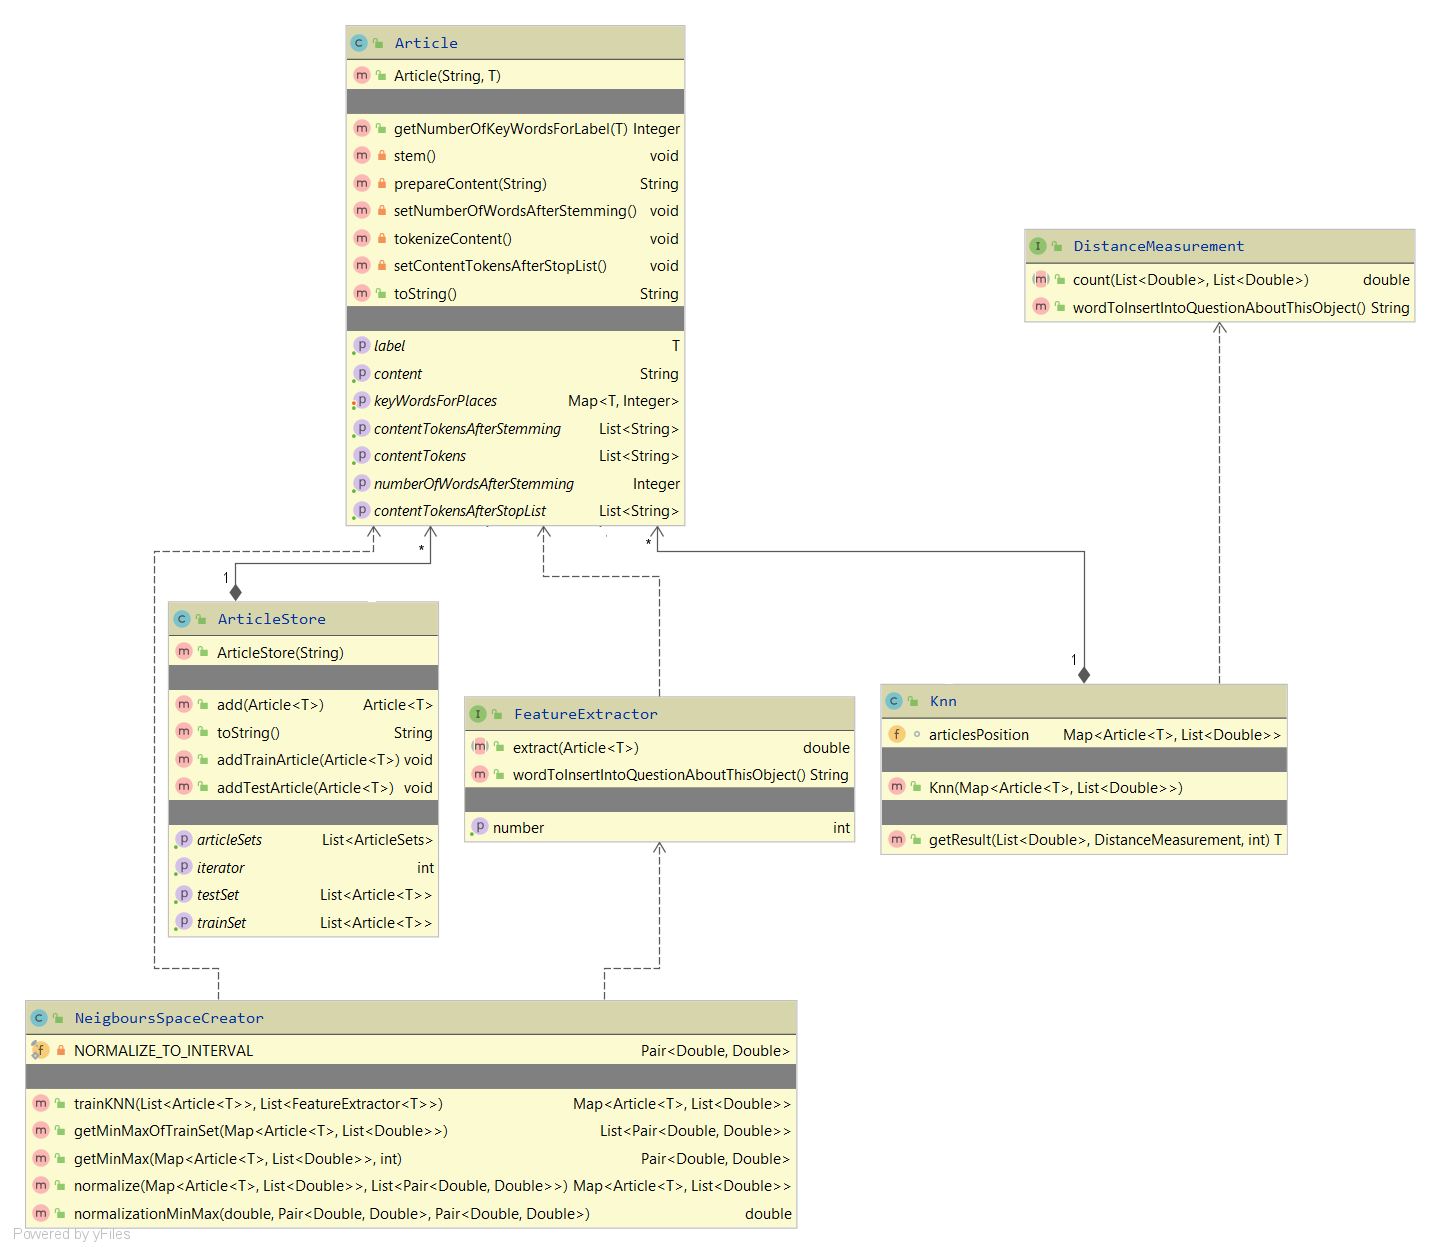
\includegraphics[width=1\textwidth]{uml}
\end{figure}
 }

\section{Materiały i metody}

{
Badania zostały przeprowadzone na zbiorze artykułów w języku angielskim które były oznaczone etykietami w dwóch kategoriach w kategorii „places” (west-germany, usa, france,uk ,canada, japan) oraz w kategorii „topics” (earn, acq) 

\subsection{Wpływ liczby sąsiadów na jakość klasyfikacji}
Badanie zostało przeprowadzone z różna ilością sąsiadów {1,3,4,7,11,12,13,19,37,59}
Pozostałe parametry były stałe:
\\*
Metryka: Metryka Euklidesa
\\*
Podział danych: 70\% - zbiór uczący (Places), 50\% - zbiór uczący (Topics)
\\*
Cechy: 1,2,3,4,5,6,7,8,9,10,11
\subsection{Wpływ podziału danych na jakość klasyfikacji}
Badanie zostało przeprowadzone z różną wielkość zbioru uczącego {30\%,40\%,50\%,60\%,70\%}
Pozostałe parametry były stałe:
\\*
Metryka: Metryka Euklidesa
\\*
Liczba sąsiadów: 37
\\*
Cechy: 1,2,3,4,5,6,7,8,9,10,11
\subsection{Wpływ metryki/miary na jakość klasyfikacji}
Badanie zostało przeprowadzone z różnymi metrykami/miarami: {Średnia arytmetyczna minimum, Metryka Czebyszewa, Metryka Euklidesa, Minimum-maximum, Metryka Uliczna, Nasza Metryka}
Pozostałe parametry były stałe:
\\*
Podział danych: 60\% - zbiór uczący (Places), 50\% - zbiór uczący (Topics)
\\*
Liczba sąsiadów: 37
\\*
Cechy: 1,2,3,4,5,6,7,8,9,10,11
\subsection{Wpływ cech na jakość klasyfikacji}
Badania zostały przeprowadzone w taki sposób, że od podstawowego zbioru cech czyli cech: 1, 2, 3, 4, 5, 6, 7, 8, 9, 10, 11 odejmowaliśmy jedną cechę (lub dodawaliśmy w przypadku cech związanych z etykietami) i najbardziej interesujące przypadki zamieściliśmy w wynikach. 
Pozostałe parametry były stałe:
\\*
Metryka: Metryka Euklidesa (Topics), Metryka Uliczna (Places)
\\*
Liczba sąsiadów: 37
\\*
Podział danych: 60\%
\subsection{Prównanie naszej metryki i metryki Czebyszewa}
Badanie zostało przeprowadzone z różna ilością sąsiadów {1,3,4,7,11,12,13,19,37,59} i przy użyci Naszej Metryki i Metryki Czebyszewa
Pozostałe parametry były stałe:
\\*
Podział danych: 60\%
\\*
Cechy: 1,2,3,4,5,6,7,8,9,10,11
}

\section{Wyniki}
{
\subsection{Wyniki klasyfikacji metodą k-NN dla 10 różnych wartości parametru k (Places)}

\begin{table}[H]
\begin{center}
\caption{Wyniki klasyfikacji dla różnej liczby sąsiadów}
\begin{tabular}{|c|c|c|c|}
\hline
\textbf{Liczba sąsiadów} & \textbf{Accuracy} & \textbf{Średni Recall} & \textbf{Średni Precision} \\ \hline
1                        & 0,697             & 0,314                  & 0,287             \\ \hline
3                        & 0,736             & 0,307                  & 0,292             \\ \hline
4                        & 0,754             & 0,311                  & 0,305             \\ \hline
7                        & 0,789             & 0,309                  & 0,363             \\ \hline
11                       & 0,807             & 0,301                  & 0,398             \\ \hline
12                       & 0,806             & 0,290                  & 0,372             \\ \hline
13                       & 0,81              & 0,291                  & 0,373             \\ \hline
19                       & 0,812             & 0,263                  & 0,364             \\ \hline
37                       & 0,814             & 0,246                  & 0,538             \\ \hline
59                       & 0,811             & 0,229                  & 0,369             \\ \hline
\end{tabular}
\end{center}
\end{table}

\begin{figure}[H]
\caption{Accuracy w zależności od liczby sąsiadów}
\centering
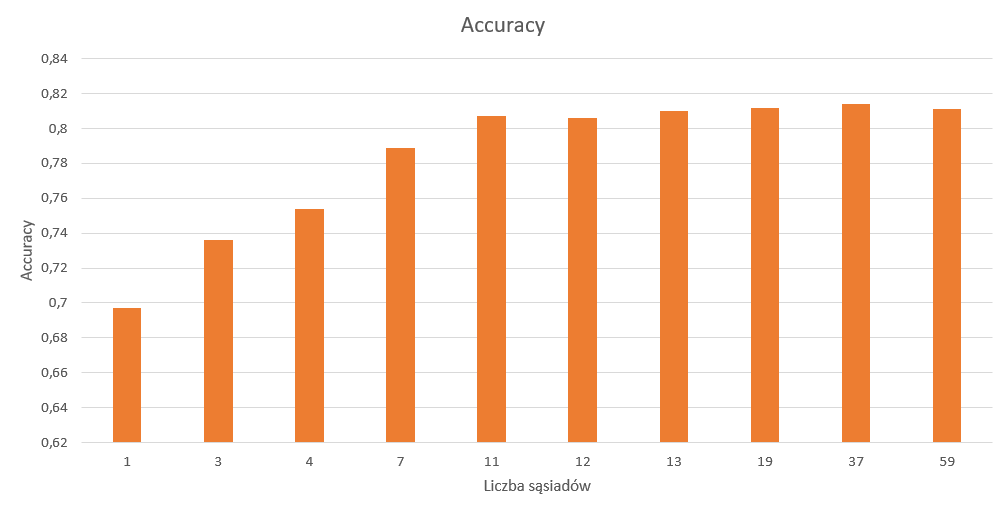
\includegraphics[width=1\textwidth]{i1}
\end{figure}

\begin{figure}[H]
\caption{Recall i Precision w zależności od liczby sąsiadów}
\centering
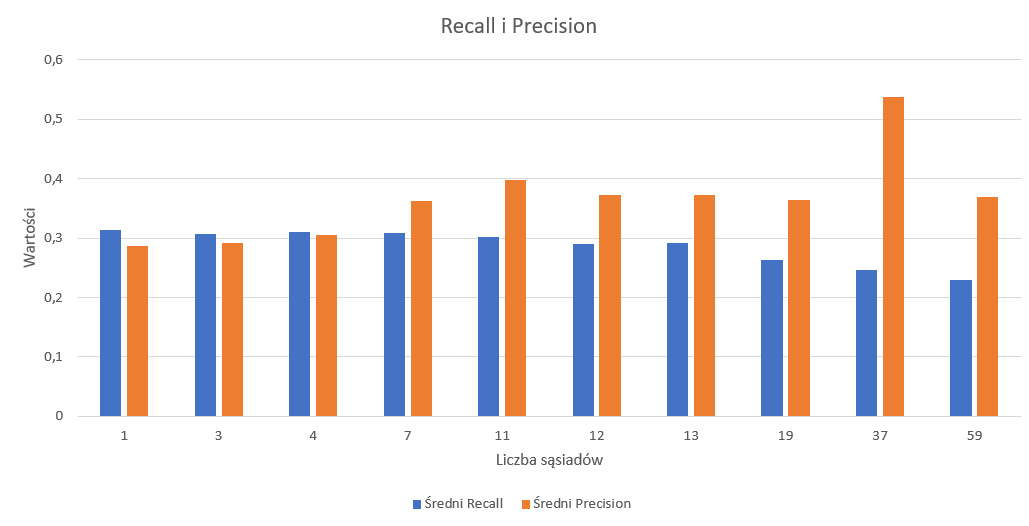
\includegraphics[width=1\textwidth]{i2}
\end{figure}

\begin{table}[H]
\begin{center}
\caption{Wyniki klasyfikacji dla różnej liczby sąsiadów z podziałem na etykiety}
\begin{tabular}{|l|l|l|l|l|l|l|}
\hline
\begin{tabular}[c]{@{}l@{}}Liczba\\ sąsiadów\end{tabular} & \begin{tabular}[c]{@{}l@{}}Recall\\ west-germany\end{tabular} & \begin{tabular}[c]{@{}l@{}}Precision\\ west-germany\end{tabular} & \begin{tabular}[c]{@{}l@{}}Recall\\ usa\end{tabular} & \begin{tabular}[c]{@{}l@{}}Precision\\ usa\end{tabular} & \begin{tabular}[c]{@{}l@{}}Recall\\ france\end{tabular} & \begin{tabular}[c]{@{}l@{}}Precision\\ france\end{tabular} \\ \hline
1                                                        & 0,16                                                          & 0,136                                                            & 0,813                                                & 0,876                                                   & 0,085                                                   & 0,054                                                      \\ \hline
3                                                        & 0,113                                                         & 0,16                                                             & 0,864                                                & 0,875                                                   & 0,017                                                   & 0,048                                                      \\ \hline
4                                                        & 0,075                                                         & 0,154                                                            & 0,886                                                & 0,875                                                   & 0,017                                                   & 0,034                                                      \\ \hline
7                                                        & 0,132                                                         & 0,326                                                            & 0,936                                                & 0,862                                                   & 0,034                                                   & 0,111                                                      \\ \hline
11                                                       & 0,075                                                         & 0,333                                                            & 0,962                                                & 0,854                                                   & 0,017                                                   & 0,111                                                      \\ \hline
12                                                       & 0,094                                                         & 0,333                                                            & 0,964                                                & 0,852                                                   & 0                                                       & 0                                                          \\ \hline
13                                                       & 0,094                                                         & 0,345                                                            & 0,969                                                & 0,853                                                   & 0                                                       & 0                                                          \\ \hline
19                                                       & 0,038                                                         & 0,25                                                             & 0,981                                                & 0,841                                                   & 0                                                       & 0                                                          \\ \hline
37                                                       & 0,028                                                         & 0,429                                                            & 0,991                                                & 0,828                                                   & 0,017                                                   & 1                                                          \\ \hline
59                                                       & 0,009                                                         & 0,143                                                            & 0,993                                                & 0,823                                                   & 0,017                                                   & 0,25                                                       \\ \hline
\end{tabular}
\end{center}
\end{table}


\begin{table}[H]
\begin{center}
\caption{Wyniki klasyfikacji dla różnej liczby sąsiadów z podziałem na etykiety}
\begin{tabular}{|l|l|l|l|l|l|l|}
\hline
\begin{tabular}[c]{@{}l@{}}Liczba\\ sąsiadów\end{tabular} & \begin{tabular}[c]{@{}l@{}}Recall \\ uk\end{tabular} & \begin{tabular}[c]{@{}l@{}}Precision\\  uk\end{tabular} & \begin{tabular}[c]{@{}l@{}}Recall\\  canada\end{tabular} & \begin{tabular}[c]{@{}l@{}}Precision\\  canada\end{tabular} & \begin{tabular}[c]{@{}l@{}}Recall\\  japan\end{tabular} & \begin{tabular}[c]{@{}l@{}}Precision\\  japan\end{tabular} \\ \hline
1                                                        & 0,332                                                & 0,298                                                   & 0,189                                                    & 0,138                                                       & 0,303                                                   & 0,219                                                      \\ \hline
3                                                        & 0,378                                                & 0,303                                                   & 0,119                                                    & 0,184                                                       & 0,352                                                   & 0,184                                                      \\ \hline
4                                                        & 0,401                                                & 0,35                                                    & 0,139                                                    & 0,179                                                       & 0,345                                                   & 0,24                                                       \\ \hline
7                                                        & 0,385                                                & 0,409                                                   & 0,057                                                    & 0,187                                                       & 0,31                                                    & 0,283                                                      \\ \hline
11                                                       & 0,378                                                & 0,478                                                   & 0,041                                                    & 0,25                                                        & 0,331                                                   & 0,361                                                      \\ \hline
12                                                       & 0,363                                                & 0,468                                                   & 0,037                                                    & 0,231                                                       & 0,283                                                   & 0,35                                                       \\ \hline
13                                                       & 0,37                                                 & 0,469                                                   & 0,025                                                    & 0,188                                                       & 0,29                                                    & 0,382                                                      \\ \hline
19                                                       & 0,332                                                & 0,503                                                   & 0,012                                                    & 0,214                                                       & 0,214                                                   & 0,378                                                      \\ \hline
37                                                       & 0,282                                                & 0,607                                                   & 0                                                        & 0                                                           & 0,159                                                   & 0,365                                                      \\ \hline
59                                                       & 0,252                                                & 0,595                                                   & 0                                                        & 0                                                           & 0,103                                                   & 0,405                                                      \\ \hline
\end{tabular}
\end{center}
\end{table}

\subsection{Wyniki klasyfikacji metodą k-NN dla 5 różnych podziałów na zbiór uczący i testowy (Places)}

\begin{table}[H]
\begin{center}
\caption{Wyniki klasyfikacji dla różnych podziałów na zbiór uczący i testowy}
\begin{tabular}{|c|c|c|c|}
\hline
\textbf{\begin{tabular}[c]{@{}c@{}}Ilość danych\\ w zbiorze uczący\end{tabular}} & \textbf{Accuracy} & \textbf{Średni Recall} & \textbf{Średni Precision} \\ \hline
30\%                                                                             & 0,811             & 0,229                  & 0,387                     \\ \hline
40\%                                                                             & 0,808             & 0,235                  & 0,369                     \\ \hline
50\%                                                                             & 0,809             & 0,240                  & 0,334                     \\ \hline
60\%                                                                             & 0,817             & 0,239                  & 0,404                     \\ \hline
70\%                                                                             & 0,814             & 0,246                  & 0,538                     \\ \hline
\end{tabular}
\end{center}
\end{table}


\begin{figure}[H]
\caption{Accuracy w zależności od podziału na zbiór uczący i testowy}
\centering
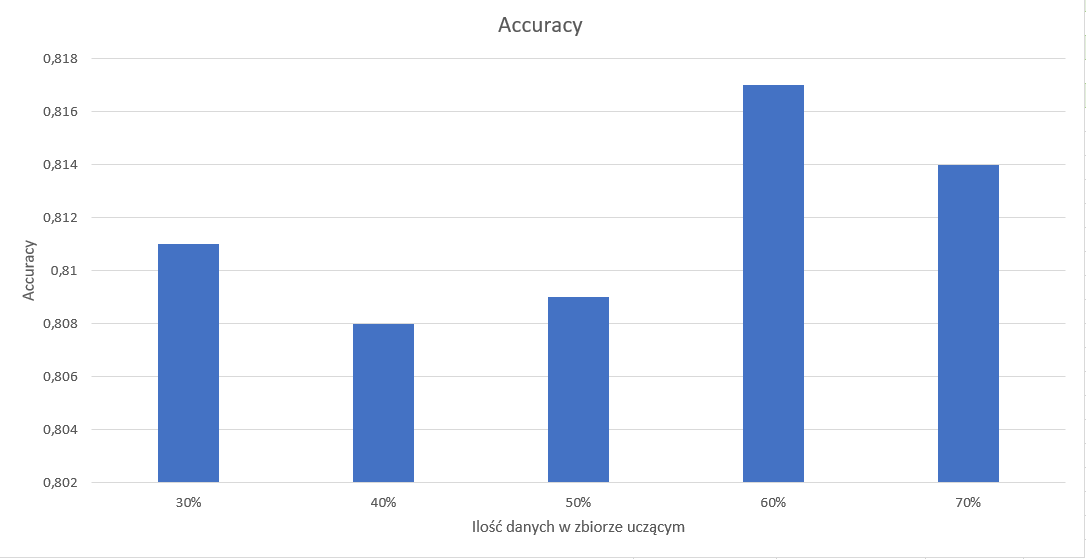
\includegraphics[width=1\textwidth]{i3}
\end{figure}

\begin{figure}[H]
\caption{Recall i Precision w zależności od podziału na zbiór uczący i testowy}
\centering
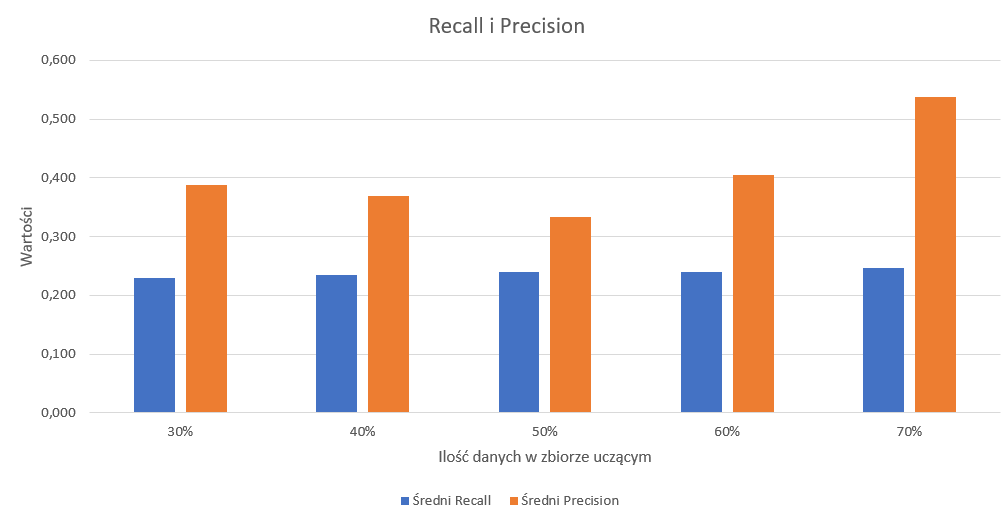
\includegraphics[width=1\textwidth]{i4}
\end{figure}


\begin{table}[H]
\begin{center}
\caption{Wyniki klasyfikacji dla różnych podziałów na zbiór uczący i testowy dla etykiet}
\begin{tabular}{|l|l|l|l|l|l|l|}
\hline
\textbf{\begin{tabular}[c]{@{}l@{}}Podział\\ danych\end{tabular}} & \textbf{\begin{tabular}[c]{@{}l@{}}Recall\\    west-germany\end{tabular}} & \textbf{\begin{tabular}[c]{@{}l@{}}Precision\\  west-germany\end{tabular}} & \textbf{\begin{tabular}[c]{@{}l@{}}Recall\\  usa\end{tabular}} & \textbf{\begin{tabular}[c]{@{}l@{}}Precision\\  usa\end{tabular}} & \textbf{\begin{tabular}[c]{@{}l@{}}Recall\\  france\end{tabular}} & \textbf{\begin{tabular}[c]{@{}l@{}}Precision \\ france\end{tabular}} \\ \hline
30\%                                                              & 0,018                                                                     & 0,444                                                                      & 0,99                                                           & 0,825                                                             & 0,019                                                             & 0,2                                                                  \\ \hline
40\%                                                              & 0,031                                                                     & 0,333                                                                      & 0,99                                                           & 0,823                                                             & 0                                                                 & 0                                                                    \\ \hline
50\%                                                              & 0,019                                                                     & 0,375                                                                      & 0,987                                                          & 0,83                                                              & 0                                                                 & 0                                                                    \\ \hline
60\%                                                              & 0,033                                                                     & 0,444                                                                      & 0,989                                                          & 0,833                                                             & 0,011                                                             & 0,25                                                                 \\ \hline
70\%                                                              & 0,028                                                                     & 0,429                                                                      & 0,991                                                          & 0,828                                                             & 0,017                                                             & 1                                                                    \\ \hline
\end{tabular}
\end{center}
\end{table}

\begin{table}[H]
\begin{center}
\caption{Wyniki klasyfikacji dla różnych podziałów na zbiór uczący i testowy dla etykiet}
\begin{tabular}{|l|l|l|l|l|l|l|}
\hline
\textbf{\begin{tabular}[c]{@{}l@{}}Podział\\ danych\end{tabular}} & \textbf{\begin{tabular}[c]{@{}l@{}}Recall\\ uk\end{tabular}} & \textbf{\begin{tabular}[c]{@{}l@{}}Precision\\  uk\end{tabular}} & \textbf{\begin{tabular}[c]{@{}l@{}}Recall\\  canada\end{tabular}} & \textbf{\begin{tabular}[c]{@{}l@{}}Precision\\  canada\end{tabular}} & \textbf{\begin{tabular}[c]{@{}l@{}}Recall\\  japan\end{tabular}} & \textbf{Precision japan} \\ \hline
30\%                                                              & 0,272                                                        & 0,561                                                            & 0                                                                 & 0                                                                    & 0,075                                                            & 0,293                    \\ \hline
40\%                                                              & 0,279                                                        & 0,515                                                            & 0                                                                 & 0                                                                    & 0,108                                                            & 0,544                    \\ \hline
50\%                                                              & 0,329                                                        & 0,536                                                            & 0                                                                 & 0                                                                    & 0,102                                                            & 0,26                     \\ \hline
60\%                                                              & 0,312                                                        & 0,558                                                            & 0                                                                 & 0                                                                    & 0,089                                                            & 0,34                     \\ \hline
70\%                                                              & 0,282                                                        & 0,607                                                            & 0                                                                 & 0                                                                    & 0,159                                                            & 0,365                    \\ \hline
\end{tabular}
\end{center}
\end{table}

\subsection{Wyniki klasyfikacji metodą k-NN dla 6 różnych metryk/miar (Places)}

\begin{table}[H]
\begin{center}
\caption{Wyniki klasyfikacji dla różnych metryk/miar}
\begin{tabular}{|c|c|c|c|}
\hline
\textbf{Metryka}             & \textbf{Accuracy} & \textbf{Średni Recall} & \textbf{Średni Precision} \\ \hline
Średnia arytmetyczna minimum & 0,819             & 0,229                  & 0,384                     \\ \hline
Metryka Czebyszewa           & 0,815             & 0,223                  & 0,379                     \\ \hline
Metryka Euklidesa            & 0,817             & 0,238                  & 0,399                     \\ \hline
Minimum-maximum              & 0,819             & 0,229                  & 0,384                     \\ \hline
Metryka Uliczna              & 0,821             & 0,242                  & 0,407                     \\ \hline
Nasza metryka                & 0,821             & 0,242                  & 0,42                      \\ \hline
\end{tabular}
\end{center}
\end{table}

\begin{figure}[H]
\caption{Accuracy w zależności od miary/metryki}
\centering
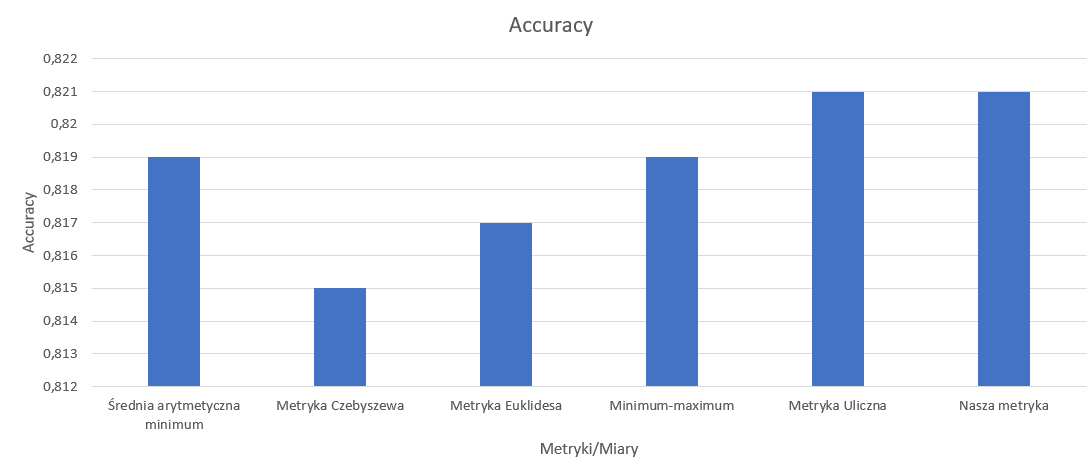
\includegraphics[width=1\textwidth]{i5}
\end{figure}

\begin{figure}[H]
\caption{Recall i Precision w zależności od miary/metryki}
\centering
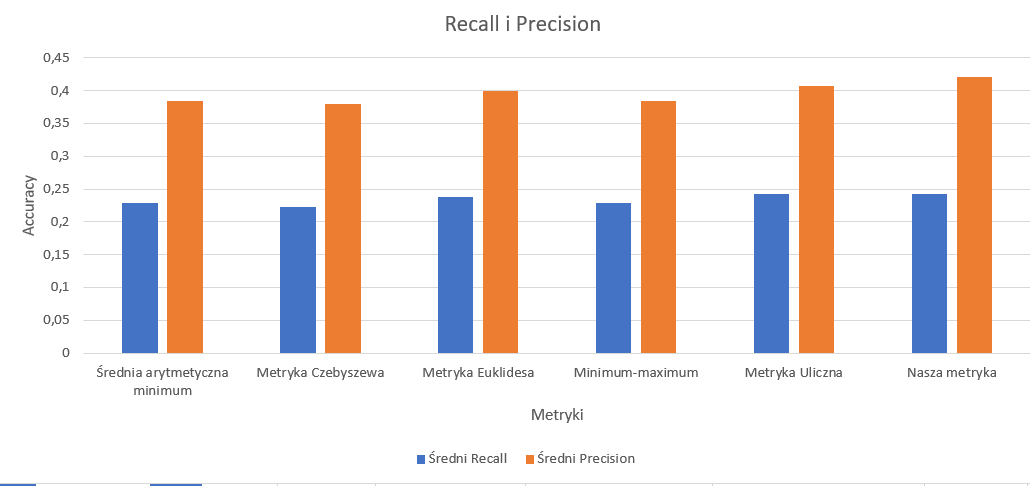
\includegraphics[width=1\textwidth]{i6}
\end{figure}

\begin{table}[H]
\begin{center}
\caption{Wyniki klasyfikacji dla różnych mair/metryk z podziałem na etykiety}
\begin{tabular}{|l|l|l|l|l|l|l|}
\hline
\textbf{Metryka}                                                           & \textbf{\begin{tabular}[c]{@{}l@{}}Recall\\ west-germany\end{tabular}} & \textbf{\begin{tabular}[c]{@{}l@{}}Precision\\ west-germany\end{tabular}} & \textbf{\begin{tabular}[c]{@{}l@{}}Recall\\ usa\end{tabular}} & \textbf{\begin{tabular}[c]{@{}l@{}}Precision\\ usa\end{tabular}} & \textbf{\begin{tabular}[c]{@{}l@{}}Recall\\ france\end{tabular}} & \textbf{\begin{tabular}[c]{@{}l@{}}Precision\\ france\end{tabular}} \\ \hline
\begin{tabular}[c]{@{}l@{}}Średnia \\ arytmetyczna\\  minimum\end{tabular} & 0,008                                                                  & 0,333                                                                     & 0,995                                                         & 0,827                                                            & 0                                                                & 0                                                                   \\ \hline
\begin{tabular}[c]{@{}l@{}}Metryka\\ Czebyszewa\end{tabular}               & 0,016                                                                  & 0,4                                                                       & 0,994                                                         & 0,825                                                            & 0                                                                & 0                                                                   \\ \hline
\begin{tabular}[c]{@{}l@{}}Metryka\\ Euklidesa\end{tabular}                & 0,033                                                                  & 0,5                                                                       & 0,989                                                         & 0,832                                                            & 0,011                                                            & 0,167                                                               \\ \hline
\begin{tabular}[c]{@{}l@{}}Minimum\\ -maximum\end{tabular}                 & 0,008                                                                  & 0,333                                                                     & 0,995                                                         & 0,827                                                            & 0                                                                & 0                                                                   \\ \hline
\begin{tabular}[c]{@{}l@{}}Metryka \\ Uliczna\end{tabular}                 & 0,016                                                                  & 0,5                                                                       & 0,994                                                         & 0,832                                                            & 0                                                                & 0                                                                   \\ \hline
\begin{tabular}[c]{@{}l@{}}Nasza\\ metryka\end{tabular}                    & 0,008                                                                  & 0,333                                                                     & 0,994                                                         & 0,83                                                             & 0,011                                                            & 0,167                                                               \\ \hline
\end{tabular}
\end{center}
\end{table}


\begin{table}[H]
\begin{center}
\caption{Wyniki klasyfikacji dla różnych mair/metryk z podziałem na etykiety}
\begin{tabular}{|l|l|l|l|l|l|l|}
\hline
\textbf{Metryka}                                                           & \textbf{\begin{tabular}[c]{@{}l@{}}Recall \\ uk\end{tabular}} & \textbf{\begin{tabular}[c]{@{}l@{}}Precision\\  uk\end{tabular}} & \textbf{\begin{tabular}[c]{@{}l@{}}Recall\\  canada\end{tabular}} & \textbf{\begin{tabular}[c]{@{}l@{}}Precision\\  canada\end{tabular}} & \textbf{\begin{tabular}[c]{@{}l@{}}Recall\\  japan\end{tabular}} & \textbf{\begin{tabular}[c]{@{}l@{}}Precision\\  japan\end{tabular}} \\ \hline
\begin{tabular}[c]{@{}l@{}}Średnia \\ arytmetyczna\\  minimum\end{tabular} & 0,271                                                         & 0,63                                                             & 0                                                                 & 0                                                                    & 0,099                                                            & 0,514                                                               \\ \hline
\begin{tabular}[c]{@{}l@{}}Metryka\\ Czebyszewa\end{tabular}               & 0,244                                                         & 0,58                                                             & 0                                                                 & 0                                                                    & 0,084                                                            & 0,471                                                               \\ \hline
\begin{tabular}[c]{@{}l@{}}Metryka\\ Euklidesa\end{tabular}                & 0,312                                                         & 0,555                                                            & 0                                                                 & 0                                                                    & 0,084                                                            & 0,34                                                                \\ \hline
\begin{tabular}[c]{@{}l@{}}Minimum\\ -maximum\end{tabular}                 & 0,271                                                         & 0,63                                                             & 0                                                                 & 0                                                                    & 0,099                                                            & 0,514                                                               \\ \hline
\begin{tabular}[c]{@{}l@{}}Metryka \\ Uliczna\end{tabular}                 & 0,3                                                           & 0,637                                                            & 0                                                                 & 0                                                                    & 0,141                                                            & 0,474                                                               \\ \hline
\begin{tabular}[c]{@{}l@{}}Nasza\\ metryka\end{tabular}                    & 0,285                                                         & 0,63                                                             & 0                                                                 & 0                                                                    & 0,152                                                            & 0,558                                                               \\ \hline
\end{tabular}
\end{center}
\end{table}


\subsection{Wyniki klasyfikacji metodą k-NN dla różnych cech (Places)}
Podstawowe cechy to 1, 2, 3, 4, 5, 6, 7, 8, 9, 10, 11
\begin{table}[H]
\begin{center}
\caption{Wyniki klasyfikacji dla 4 podzbiorów cech}
\begin{tabular}{|c|c|c|c|}
\hline
\textbf{\begin{tabular}[c]{@{}c@{}}Różnice pomiędzy \\ cechami podstawowymi\end{tabular}} & \textbf{Accuracy} & \textbf{Średni Recall} & \textbf{Średni Precision} \\ \hline
Cechy podstawowe                                                                          & 0,817             & 0,238                  & 0,399                     \\ \hline
\begin{tabular}[c]{@{}c@{}}Dodatkowe cechy:\\ 12 13 14 15 16 17\end{tabular}              & 0,875             & 0,492                  & 0,892                     \\ \hline
Brak cechy 8                                                                              & 0,805             & 0,179                  & 0,25                      \\ \hline
Brak cechy 6                                                                              & 0,811             & 0,22                   & 0,351                     \\ \hline
Brak cechy 9                                                                              & 0,819             & 0,241                  & 0,417                     \\ \hline
\end{tabular}
\end{center}
\end{table}


\begin{table}[H]
\begin{center}
\caption{Wyniki klasyfikacji dla 4 podzbiorów cech z podziałem na etykiety}
\begin{tabular}{|l|l|l|l|l|l|l|}
\hline
\textbf{\begin{tabular}[c]{@{}l@{}}Różnice\\ w cechach\end{tabular}}    & \textbf{\begin{tabular}[c]{@{}l@{}}Recall\\ west-germany\end{tabular}} & \textbf{\begin{tabular}[c]{@{}l@{}}Precision\\ west-germany\end{tabular}} & \textbf{\begin{tabular}[c]{@{}l@{}}Recall\\ usa\end{tabular}} & \textbf{\begin{tabular}[c]{@{}l@{}}Precision\\ usa\end{tabular}} & \textbf{\begin{tabular}[c]{@{}l@{}}Recall\\ france\end{tabular}} & \textbf{\begin{tabular}[c]{@{}l@{}}Precision\\ france\end{tabular}} \\ \hline
\begin{tabular}[c]{@{}l@{}}Cechy\\ podstawowe\end{tabular}              & 0,033                                                                  & 0,5                                                                       & 0,989                                                         & 0,832                                                            & 0,011                                                            & 0,167                                                               \\ \hline
\begin{tabular}[c]{@{}l@{}}Dodatkowo\\ 12 13 14\\ 15 16 17\end{tabular} & 0,325                                                                  & 0,952                                                                     & 0,995                                                         & 0,873                                                            & 0,389                                                            & 0,833                                                               \\ \hline
Brak 8                                                                  & 0                                                                      & 0                                                                         & 0,998                                                         & 0,806                                                            & 0                                                                & 0                                                                   \\ \hline
Brak 6                                                                  & 0,024                                                                  & 0,429                                                                     & 0,99                                                          & 0,825                                                            & 0                                                                & 0                                                                   \\ \hline
Brak 9                                                                  & 0,033                                                                  & 0,5                                                                       & 0,991                                                         & 0,833                                                            & 0,011                                                            & 0,2                                                                 \\ \hline
\end{tabular}
\end{center}
\end{table}



\begin{table}[H]
\begin{center}
\caption{Wyniki klasyfikacji dla 4 podzbiorów cech z podziałem na etykiety}
\begin{tabular}{|l|l|l|l|l|l|l|}
\hline
\textbf{\begin{tabular}[c]{@{}l@{}}Różnice\\ w cechach\end{tabular}}    & \textbf{\begin{tabular}[c]{@{}l@{}}Recall\\ uk\end{tabular}} & \textbf{\begin{tabular}[c]{@{}l@{}}Precision\\ uk\end{tabular}} & \textbf{\begin{tabular}[c]{@{}l@{}}Recall\\ canada\end{tabular}} & \textbf{\begin{tabular}[c]{@{}l@{}}Precision\\ canada\end{tabular}} & \textbf{\begin{tabular}[c]{@{}l@{}}Recall\\ japan\end{tabular}} & \textbf{\begin{tabular}[c]{@{}l@{}}Precision\\ japan\end{tabular}} \\ \hline
\begin{tabular}[c]{@{}l@{}}Cechy\\ podstawowe\end{tabular}              & 0,312                                                        & 0,555                                                           & 0                                                                & 0                                                                   & 0,084                                                           & 0,34                                                               \\ \hline
\begin{tabular}[c]{@{}l@{}}Dodatkowo\\ 12 13 14\\ 15 16 17\end{tabular} & 0,468                                                        & 0,874                                                           & 0,254                                                            & 0,86                                                                & 0,524                                                           & 0,962                                                              \\ \hline
Brak 8                                                                  & 0,074                                                        & 0,694                                                           & 0                                                                & 0                                                                   & 0                                                               & 0                                                                  \\ \hline
Brak 6                                                                  & 0,212                                                        & 0,514                                                           & 0                                                                & 0                                                                   & 0,094                                                           & 0,34                                                               \\ \hline
Brak 9                                                                  & 0,321                                                        & 0,565                                                           & 0                                                                & 0                                                                   & 0,089                                                           & 0,405                                                              \\ \hline
\end{tabular}
\end{center}
\end{table}



\subsection{Wyniki klasyfikacji metodą k-NN dla 10 różnych wartości parametru k}

\begin{table}[H]
\begin{center}
\caption{Wyniki klasyfikacji dla różnej liczby sąsiadów (Topics)}
\begin{tabular}{|c|c|c|c|}
\hline
\textbf{Liczba sąsiadów} & \textbf{Accuracy} & \textbf{Średni Recall} & \textbf{Średni Precision} \\ \hline
1                        & 0,87              & 0,86                   & 0,859                     \\ \hline
3                        & 0,892             & 0,889                  & 0,881                     \\ \hline
4                        & 0,896             & 0,905                  & 0,883                     \\ \hline
7                        & 0,907             & 0,907                  & 0,896                     \\ \hline
11                       & 0,914             & 0,917                  & 0,902                     \\ \hline
12                       & 0,914             & 0,921                  & 0,902                     \\ \hline
13                       & 0,912             & 0,916                  & 0,901                     \\ \hline
19                       & 0,913             & 0,918                  & 0,902                     \\ \hline
37                       & 0,917             & 0,925                  & 0,905                     \\ \hline
59                       & 0,911             & 0,922                  & 0,899                     \\ \hline
\end{tabular}
\end{center}
\end{table}

\begin{figure}[H]
\caption{Accuracy w zależności od liczby sąsiadów}
\centering
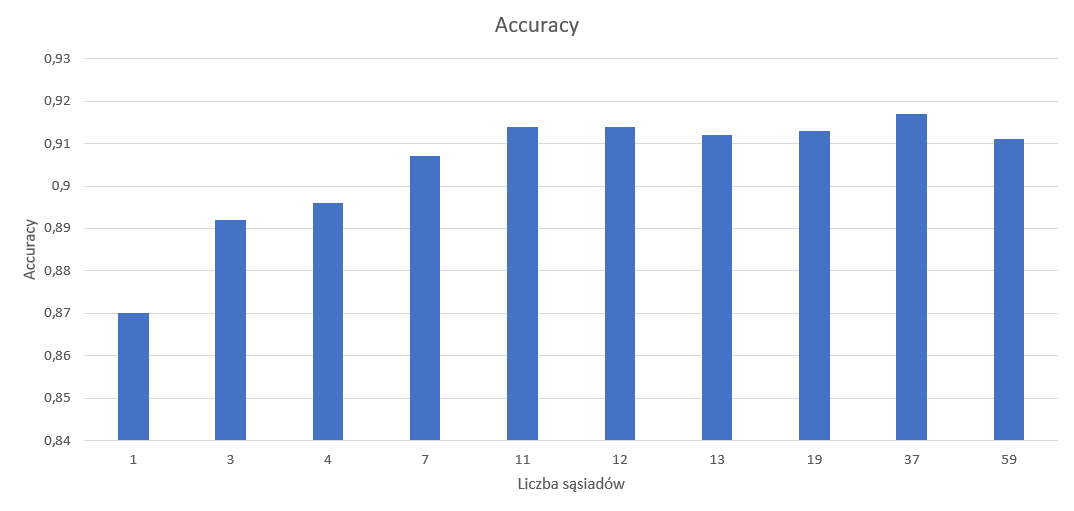
\includegraphics[width=1\textwidth]{i7}
\end{figure}

\begin{figure}[H]
\caption{Recall i Precision w zależności od liczby sąsiadów}
\centering
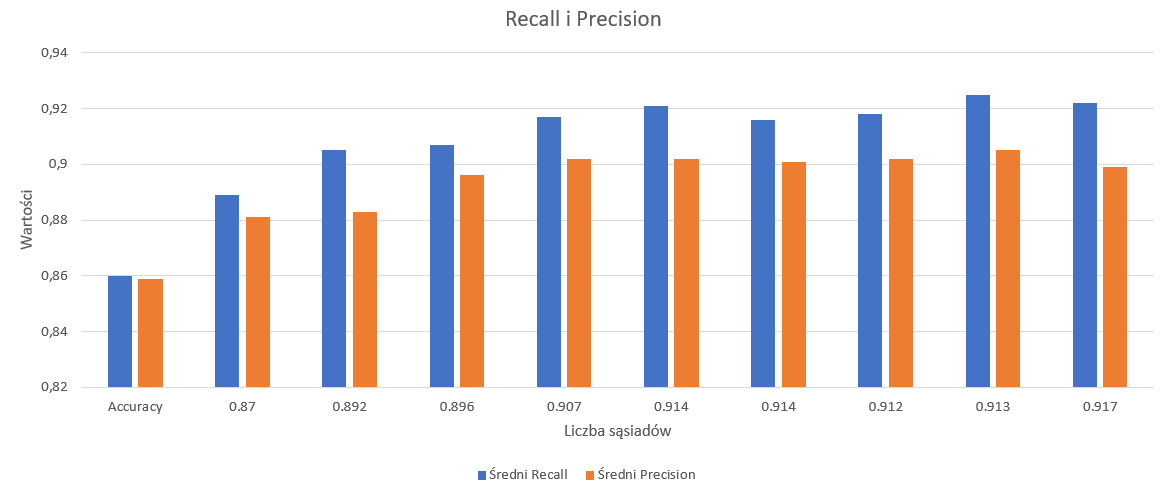
\includegraphics[width=1\textwidth]{i8}
\end{figure}

\begin{table}[H]
\begin{center}
\caption{Wyniki klasyfikacji dla różnej liczby sąsiadów z podziałem na etykiety}
\begin{tabular}{|l|l|l|l|l|}
\hline
\textbf{Liczba sąsiadów} & \textbf{Recall earn} & \textbf{Precision earn} & \textbf{Recall acq} & \textbf{Precision acq} \\ \hline
1                        & 0,897                & 0,899                   & 0,822               & 0,819                  \\ \hline
3                        & 0,901                & 0,928                   & 0,877               & 0,834                  \\ \hline
4                        & 0,873                & 0,96                    & 0,936               & 0,807                  \\ \hline
7                        & 0,906                & 0,946                   & 0,908               & 0,845                  \\ \hline
11                       & 0,906                & 0,957                   & 0,928               & 0,847                  \\ \hline
12                       & 0,894                & 0,968                   & 0,948               & 0,835                  \\ \hline
13                       & 0,902                & 0,958                   & 0,93                & 0,843                  \\ \hline
19                       & 0,901                & 0,961                   & 0,935               & 0,843                  \\ \hline
37                       & 0,898                & 0,97                    & 0,951               & 0,841                  \\ \hline
59                       & 0,884                & 0,974                   & 0,959               & 0,824                  \\ \hline
\end{tabular}
\end{center}
\end{table}

\subsection{Wyniki klasyfikacji metodą k-NN dla 5 różnych podziałów na zbiór uczący i testowy (Topics)}

\begin{table}[H]
\begin{center}
\caption{Wyniki klasyfikacji dla różnych podziałów na zbiór uczący i testowy}
\begin{tabular}{|c|c|c|c|}
\hline
\textbf{Podział danych} & \textbf{Accuracy} & \textbf{Średni Recall} & \textbf{Średni Precision} \\ \hline
30,00\%                 & 0,912             & 0,921                  & 0,901                     \\ \hline
40,00\%                 & 0,906             & 0,921                  & 0,893                     \\ \hline
50,00\%                 & 0,917             & 0,925                  & 0,905                     \\ \hline
60,00\%                 & 0,921             & 0,926                  & 0,909                     \\ \hline
70,00\%                 & 0,915             & 0,925                  & 0,902                     \\ \hline
\end{tabular}
\end{center}
\end{table}


\begin{figure}[H]
\caption{Accuracy w zależności od podziału na zbiór uczący i testowy}
\centering
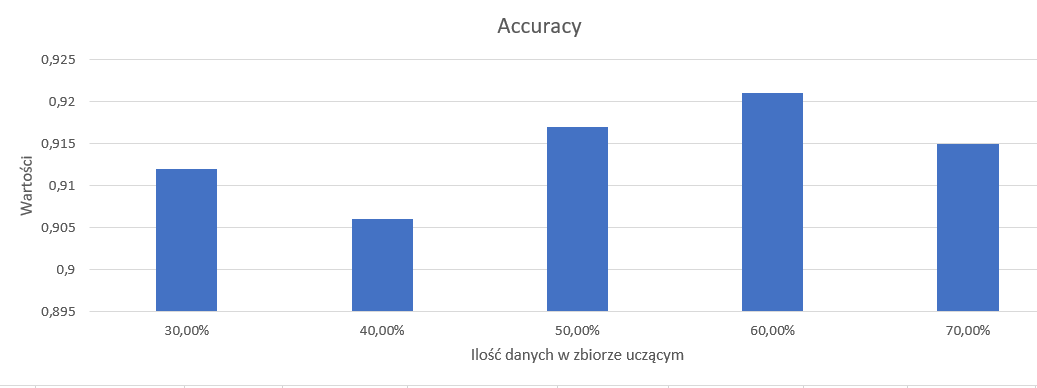
\includegraphics[width=1\textwidth]{i11}
\end{figure}

\begin{figure}[H]
\caption{Recall i Precision w zależności od podziału na zbiór uczący i testowy}
\centering
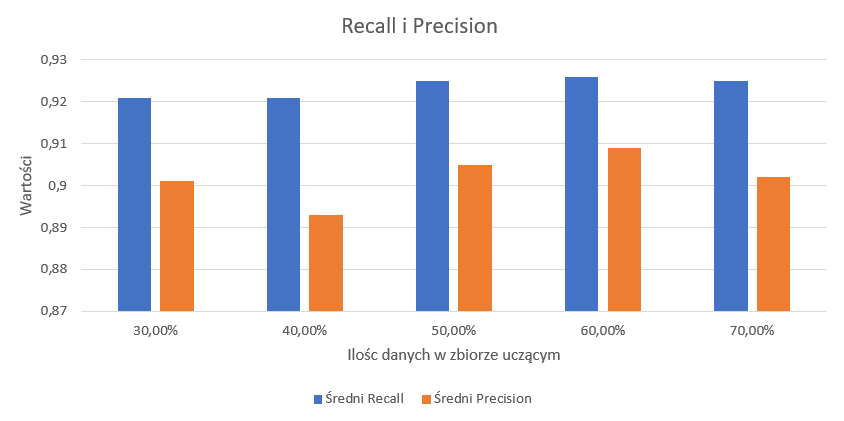
\includegraphics[width=1\textwidth]{i12}
\end{figure}

\begin{table}[H]
\begin{center}
\caption{Wyniki klasyfikacji dla różnych podziałów na zbiór uczący i testowy dla różnych etykiet}
\begin{tabular}{|l|l|l|l|l|}
\hline
\textbf{\begin{tabular}[c]{@{}l@{}}Podział \\ danych\end{tabular}} & \textbf{\begin{tabular}[c]{@{}l@{}}Recall \\  west-germany\end{tabular}} & \textbf{\begin{tabular}[c]{@{}l@{}}Precision\\  west-germany\end{tabular}} & \textbf{\begin{tabular}[c]{@{}l@{}}Recall\\  usa\end{tabular}} & \textbf{Precision usa} \\ \hline
30,00\%                                                            & 0,018                                                                    & 0,444                                                                      & 0,99                                                           & 0,825                  \\ \hline
40,00\%                                                            & 0,031                                                                    & 0,333                                                                      & 0,99                                                           & 0,823                  \\ \hline
50,00\%                                                            & 0,019                                                                    & 0,375                                                                      & 0,987                                                          & 0,83                   \\ \hline
60,00\%                                                            & 0,033                                                                    & 0,444                                                                      & 0,989                                                          & 0,833                  \\ \hline
70,00\%                                                            & 0,028                                                                    & 0,429                                                                      & 0,991                                                          & 0,828                  \\ \hline
\end{tabular}
\end{center}
\end{table}


\subsection{Wyniki klasyfikacji metodą k-NN dla 6 różnych metryk/miar (Topics)}

\begin{table}[H]
\begin{center}
\caption{Wyniki klasyfikacji dla różnych metryk/miar}
\begin{tabular}{|c|c|c|c|}
\hline
\textbf{Metryka}             & \textbf{Accuracy} & \textbf{Średni Recall} & \textbf{Średni Precision} \\ \hline
Średnia arytmetyczna minimum & 0,905             & 0,918                  & 0,893                     \\ \hline
Metryka Czebyszewa           & 0,911             & 0,919                  & 0,899                     \\ \hline
Metryka Euklidesa            & 0,917             & 0,925                  & 0,905                     \\ \hline
Minimum-maximum              & 0,905             & 0,918                  & 0,893                     \\ \hline
Metryka Uliczna              & 0,911             & 0,92                   & 0,899                     \\ \hline
Nasza metryka                & 0,907             & 0,916                  & 0,894                     \\ \hline
\end{tabular}
\end{center}
\end{table}

\begin{figure}[H]
\caption{Accuracy w zależności od miary/metryki}
\centering
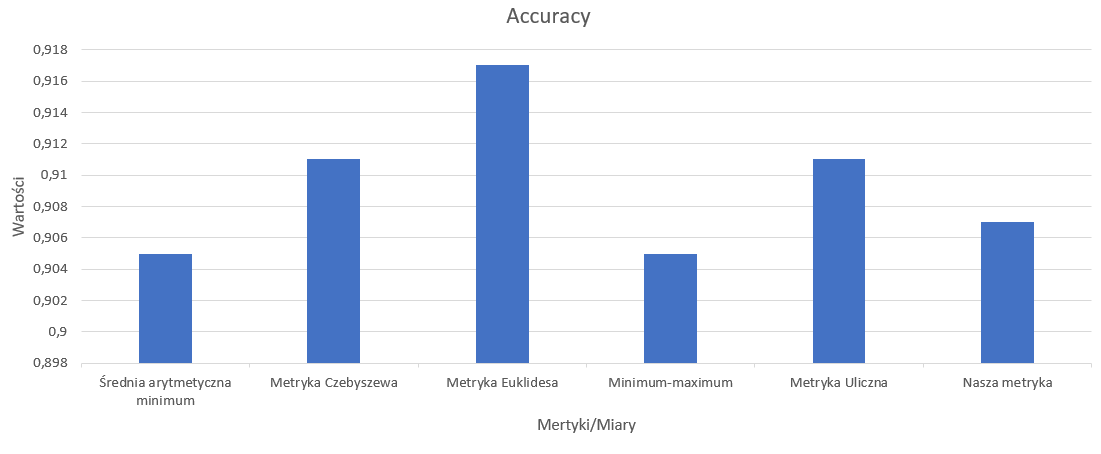
\includegraphics[width=1\textwidth]{i9}
\end{figure}

\begin{figure}[H]
\caption{Recall i Precision w zależności od miary/metryki}
\centering
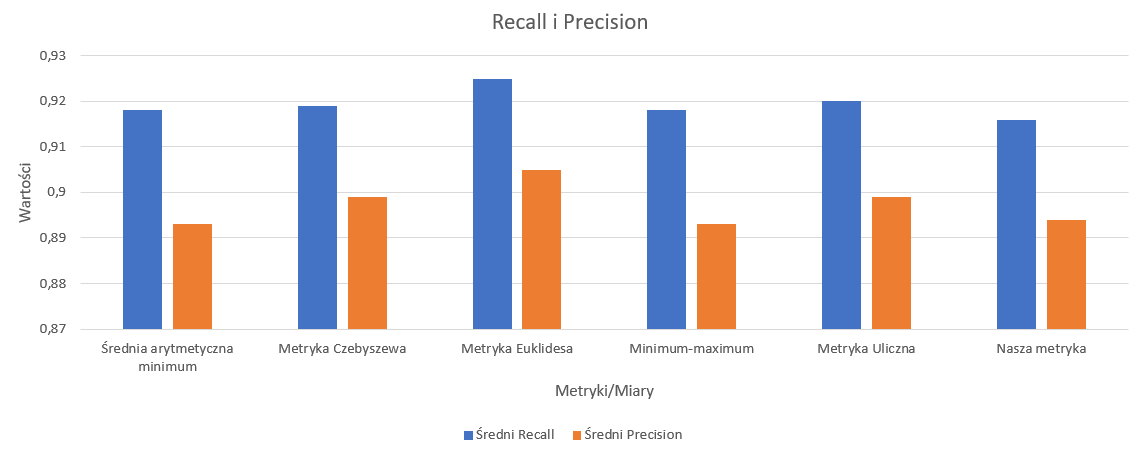
\includegraphics[width=1\textwidth]{i10}
\end{figure}

\begin{table}[H]
\begin{center}
\caption{Wyniki klasyfikacji dla różnych metryk z podziałem na etykiet}
\begin{tabular}{|l|l|l|l|l|}
\hline
\textbf{Metryka}                                                         & \textbf{Recall earn} & \textbf{Precision earn} & \textbf{Recall acq} & \textbf{Precision acq} \\ \hline
\begin{tabular}[c]{@{}l@{}}Średnia\\ arytmetyczna\\ minimum\end{tabular} & 0,871                & 0,978                   & 0,966               & 0,809                  \\ \hline
\begin{tabular}[c]{@{}l@{}}Metryka\\ Czebyszewa\end{tabular}             & 0,89                 & 0,968                   & 0,947               & 0,829                  \\ \hline
\begin{tabular}[c]{@{}l@{}}Metryka\\ Euklidesa\end{tabular}              & 0,898                & 0,97                    & 0,951               & 0,841                  \\ \hline
\begin{tabular}[c]{@{}l@{}}Minimum\\ -maximum\end{tabular}               & 0,871                & 0,978                   & 0,966               & 0,809                  \\ \hline
\begin{tabular}[c]{@{}l@{}}Metryka\\ Uliczna\end{tabular}                & 0,887                & 0,971                   & 0,953               & 0,826                  \\ \hline
\begin{tabular}[c]{@{}l@{}}Nasza\\ metryka\end{tabular}                  & 0,882                & 0,969                   & 0,949               & 0,82                   \\ \hline
\end{tabular}
\end{center}
\end{table}

\subsection{Wyniki klasyfikacji metodą k-NN dla różnych cech (Topics)}

Podstawowe cechy to 1, 2, 3, 4, 5, 6, 7, 8, 9, 10, 11

\begin{table}[H]
\begin{center}
\caption{Wyniki klasyfikacji dla 4 podzbiorów cech}
\begin{tabular}{|c|c|c|c|}
\hline
\textbf{\begin{tabular}[c]{@{}c@{}}Różnice pomiędzy \\ cechami podstawowymi\end{tabular}} & \textbf{Accuracy} & \textbf{Średni Recall} & \textbf{Średni Precision} \\ \hline
Cechy podstawowe                                                                          & 0,921             & 0,926                  & 0,909                     \\ \hline
Dodatkowe cechy: 12 13                                                                    & 0,938             & 0,944                  & 0,926                     \\ \hline
Brak cechy 11                                                                             & 0,894             & 0,899                  & 0,88                      \\ \hline
Brak cechy 3                                                                              & 0,871             & 0,888                  & 0,861                     \\ \hline
Brak cechy 10                                                                             & 0,925             & 0,928                  & 0,913                     \\ \hline
\end{tabular}
\end{center}
\end{table}


\begin{table}[H]
\begin{center}
\caption{Wyniki klasyfikacji dla 4 podzbiorów cech z podziałem na etykiety}
\begin{tabular}{|l|l|l|l|l|}
\hline
\textbf{\begin{tabular}[c]{@{}l@{}}Różnice\\ w cechach\end{tabular}} & \textbf{\begin{tabular}[c]{@{}l@{}}Recall\\ earn\end{tabular}} & \textbf{\begin{tabular}[c]{@{}l@{}}Precision\\ earn\end{tabular}} & \textbf{\begin{tabular}[c]{@{}l@{}}Recall\\ acq\end{tabular}} & \textbf{\begin{tabular}[c]{@{}l@{}}Precision\\ acq\end{tabular}} \\ \hline
Podstawowe                                                           & 0,909                                                          & 0,966                                                             & 0,943                                                         & 0,852                                                            \\ \hline
\begin{tabular}[c]{@{}l@{}}Dodatkowo\\ 12 13\end{tabular}            & 0,921                                                          & 0,981                                                             & 0,967                                                         & 0,872                                                            \\ \hline
Brak 11                                                              & 0,879                                                          & 0,951                                                             & 0,919                                                         & 0,809                                                            \\ \hline
Brak 3                                                               & 0,829                                                          & 0,966                                                             & 0,948                                                         & 0,755                                                            \\ \hline
Brak 10                                                              & 0,917                                                          & 0,964                                                             & 0,938                                                         & 0,863                                                            \\ \hline
\end{tabular}
\end{center}
\end{table}

\subsection{Porównanie naszej metryki z metryką Czebyszewa  (Places)}

\begin{table}[H]
\begin{center}
\caption{Wyniki klasyfikacji dla różnej liczby sąsiadów}
\begin{tabular}{|c|c|c|}
\hline
\textbf{Liczba sąsiadów} & \textbf{\begin{tabular}[c]{@{}c@{}}Accuracy \\ Nasza Metryka\end{tabular}} & \textbf{\begin{tabular}[c]{@{}c@{}}Accuracy\\ Metryka Czebyszewa\end{tabular}} \\ \hline
1                        & 0,701                                                                      & 0,694                                                                          \\ \hline
3                        & 0,751                                                                      & 0,735                                                                          \\ \hline
4                        & 0,763                                                                      & 0,749                                                                          \\ \hline
7                        & 0,802                                                                      & 0,79                                                                           \\ \hline
11                       & 0,816                                                                      & 0,803                                                                          \\ \hline
12                       & 0,816                                                                      & 0,804                                                                          \\ \hline
13                       & 0,816                                                                      & 0,806                                                                          \\ \hline
19                       & 0,819                                                                      & 0,813                                                                          \\ \hline
37                       & 0,821                                                                      & 0,815                                                                          \\ \hline
59                       & 0,817                                                                      & 0,814                                                                          \\ \hline
\end{tabular}
\end{center}
\end{table}

\begin{table}[H]
\begin{center}
\caption{Wyniki klasyfikacji dla różnej liczby sąsiadów z podziałem na etykiety (Nasza metryka)}
\begin{tabular}{|l|l|l|l|l|l|l|}
\hline
\textbf{\begin{tabular}[c]{@{}l@{}}Liczba\\ sąsiadów\end{tabular}} & \textbf{\begin{tabular}[c]{@{}l@{}}Recall\\ west-germany\end{tabular}} & \textbf{\begin{tabular}[c]{@{}l@{}}Precision\\ west-germany\end{tabular}} & \textbf{\begin{tabular}[c]{@{}l@{}}Recall\\ usa\end{tabular}} & \textbf{\begin{tabular}[c]{@{}l@{}}Precision\\ usa\end{tabular}} & \textbf{\begin{tabular}[c]{@{}l@{}}Recall\\ france\end{tabular}} & \textbf{\begin{tabular}[c]{@{}l@{}}Precision\\  france\end{tabular}} \\ \hline
1                                                                  & 0,171                                                                  & 0,149                                                                     & 0,808                                                         & 0,883                                                            & 0,111                                                            & 0,075                                                                \\ \hline
3                                                                  & 0,081                                                                  & 0,204                                                                     & 0,882                                                         & 0,885                                                            & 0,156                                                            & 0,083                                                                \\ \hline
4                                                                  & 0,098                                                                  & 0,231                                                                     & 0,897                                                         & 0,879                                                            & 0,078                                                            & 0,062                                                                \\ \hline
7                                                                  & 0,057                                                                  & 0,179                                                                     & 0,952                                                         & 0,866                                                            & 0,1                                                              & 0,155                                                                \\ \hline
11                                                                 & 0,049                                                                  & 0,261                                                                     & 0,973                                                         & 0,856                                                            & 0,089                                                            & 0,216                                                                \\ \hline
12                                                                 & 0,033                                                                  & 0,2                                                                       & 0,974                                                         & 0,854                                                            & 0,089                                                            & 0,235                                                                \\ \hline
13                                                                 & 0,049                                                                  & 0,353                                                                     & 0,975                                                         & 0,851                                                            & 0,056                                                            & 0,185                                                                \\ \hline
19                                                                 & 0,024                                                                  & 0,273                                                                     & 0,985                                                         & 0,843                                                            & 0,044                                                            & 0,222                                                                \\ \hline
37                                                                 & 0,008                                                                  & 0,333                                                                     & 0,994                                                         & 0,83                                                             & 0,011                                                            & 0,167                                                                \\ \hline
59                                                                 & 0                                                                      & 0                                                                         & 0,998                                                         & 0,821                                                            & 0                                                                & 0                                                                    \\ \hline
\end{tabular}
\end{center}
\end{table}

\begin{table}[H]
\begin{center}
\caption{Wyniki klasyfikacji dla różnej liczby sąsiadów z podziałem na etykiety (Nasza Metryka)}
\begin{tabular}{|l|l|l|l|l|l|l|}
\hline
\textbf{\begin{tabular}[c]{@{}l@{}}Liczba\\ sąsiadów\end{tabular}} & \textbf{\begin{tabular}[c]{@{}l@{}}Recall\\ uk\end{tabular}} & \textbf{\begin{tabular}[c]{@{}l@{}}Precision\\ uk\end{tabular}} & \textbf{\begin{tabular}[c]{@{}l@{}}Recall\\ canada\end{tabular}} & \textbf{\begin{tabular}[c]{@{}l@{}}Precision\\ canada\end{tabular}} & \textbf{\begin{tabular}[c]{@{}l@{}}Recall\\ japan\end{tabular}} & \textbf{\begin{tabular}[c]{@{}l@{}}Precision\\ japan\end{tabular}} \\ \hline
1                                                                  & 0,382                                                        & 0,297                                                           & 0,187                                                            & 0,125                                                               & 0,33                                                            & 0,267                                                              \\ \hline
3                                                                  & 0,335                                                        & 0,376                                                           & 0,165                                                            & 0,141                                                               & 0,236                                                           & 0,241                                                              \\ \hline
4                                                                  & 0,368                                                        & 0,379                                                           & 0,152                                                            & 0,155                                                               & 0,204                                                           & 0,235                                                              \\ \hline
7                                                                  & 0,374                                                        & 0,439                                                           & 0,076                                                            & 0,224                                                               & 0,215                                                           & 0,293                                                              \\ \hline
11                                                                 & 0,365                                                        & 0,506                                                           & 0,057                                                            & 0,273                                                               & 0,194                                                           & 0,349                                                              \\ \hline
12                                                                 & 0,359                                                        & 0,508                                                           & 0,06                                                             & 0,311                                                               & 0,194                                                           & 0,352                                                              \\ \hline
13                                                                 & 0,365                                                        & 0,512                                                           & 0,044                                                            & 0,311                                                               & 0,178                                                           & 0,327                                                              \\ \hline
19                                                                 & 0,324                                                        & 0,545                                                           & 0,029                                                            & 0,375                                                               & 0,178                                                           & 0,405                                                              \\ \hline
37                                                                 & 0,285                                                        & 0,63                                                            & 0                                                                & 0                                                                   & 0,152                                                           & 0,558                                                              \\ \hline
59                                                                 & 0,232                                                        & 0,681                                                           & 0                                                                & 0                                                                   & 0,058                                                           & 0,611                                                              \\ \hline
\end{tabular}
\end{center}
\end{table}

\begin{table}[H]
\begin{center}
\caption{Wyniki klasyfikacji dla różnej liczby sąsiadów z podziałem na etykiety (Metryka Czebyszewa)}
\begin{tabular}{|l|l|l|l|l|l|l|}
\hline
\textbf{\begin{tabular}[c]{@{}l@{}}Liczba\\ sąsiadów\end{tabular}} & \textbf{\begin{tabular}[c]{@{}l@{}}Recall\\ west-germany\end{tabular}} & \textbf{\begin{tabular}[c]{@{}l@{}}Precision\\ west-germany\end{tabular}} & \textbf{\begin{tabular}[c]{@{}l@{}}Recall\\ usa\end{tabular}} & \textbf{\begin{tabular}[c]{@{}l@{}}Precision\\ usa\end{tabular}} & \textbf{\begin{tabular}[c]{@{}l@{}}Recall\\ france\end{tabular}} & \textbf{\begin{tabular}[c]{@{}l@{}}Precision\\ france\end{tabular}} \\ \hline
1                                                                  & 0,179                                                                  & 0,142                                                                     & 0,807                                                         & 0,875                                                            & 0,089                                                            & 0,066                                                               \\ \hline
3                                                                  & 0,089                                                                  & 0,224                                                                     & 0,866                                                         & 0,878                                                            & 0,089                                                            & 0,052                                                               \\ \hline
4                                                                  & 0,114                                                                  & 0,255                                                                     & 0,884                                                         & 0,868                                                            & 0,1                                                              & 0,087                                                               \\ \hline
7                                                                  & 0,081                                                                  & 0,27                                                                      & 0,944                                                         & 0,856                                                            & 0,078                                                            & 0,091                                                               \\ \hline
11                                                                 & 0,065                                                                  & 0,242                                                                     & 0,964                                                         & 0,847                                                            & 0,033                                                            & 0,088                                                               \\ \hline
12                                                                 & 0,041                                                                  & 0,208                                                                     & 0,969                                                         & 0,843                                                            & 0,022                                                            & 0,061                                                               \\ \hline
13                                                                 & 0,024                                                                  & 0,167                                                                     & 0,973                                                         & 0,843                                                            & 0                                                                & 0                                                                   \\ \hline
19                                                                 & 0,049                                                                  & 0,316                                                                     & 0,983                                                         & 0,838                                                            & 0,011                                                            & 0,062                                                               \\ \hline
37                                                                 & 0,016                                                                  & 0,4                                                                       & 0,994                                                         & 0,825                                                            & 0                                                                & 0                                                                   \\ \hline
59                                                                 & 0                                                                      & 0                                                                         & 0,997                                                         & 0,82                                                             & 0                                                                & 0                                                                   \\ \hline
\end{tabular}
\end{center}
\end{table}


\begin{table}[H]
\begin{center}
\caption{Wyniki klasyfikacji dla różnej liczby sąsiadów z podziałem na etykiety (Metryka Czebyszewa)}
\begin{tabular}{|l|l|l|l|l|l|l|}
\hline
\begin{tabular}[c]{@{}l@{}}Liczba\\ sąsiadów\end{tabular} & \begin{tabular}[c]{@{}l@{}}Recall\\ uk\end{tabular} & \begin{tabular}[c]{@{}l@{}}Precision\\ uk\end{tabular} & \begin{tabular}[c]{@{}l@{}}Recall\\ canada\end{tabular} & \begin{tabular}[c]{@{}l@{}}Precision\\ canada\end{tabular} & \begin{tabular}[c]{@{}l@{}}Recall\\ japan\end{tabular} & \begin{tabular}[c]{@{}l@{}}Precision\\ japan\end{tabular} \\ \hline
1                                                         & 0,261                                               & 0,159                                                  & 0,114                                                   & 0,309                                                      & 0,245                                                  & 0,267                                                     \\ \hline
3                                                         & 0,309                                               & 0,152                                                  & 0,134                                                   & 0,225                                                      & 0,207                                                  & 0,241                                                     \\ \hline
4                                                         & 0,325                                               & 0,124                                                  & 0,132                                                   & 0,209                                                      & 0,227                                                  & 0,235                                                     \\ \hline
7                                                         & 0,422                                               & 0,051                                                  & 0,165                                                   & 0,162                                                      & 0,215                                                  & 0,293                                                     \\ \hline
11                                                        & 0,466                                               & 0,019                                                  & 0,146                                                   & 0,178                                                      & 0,276                                                  & 0,349                                                     \\ \hline
12                                                        & 0,473                                               & 0,016                                                  & 0,167                                                   & 0,162                                                      & 0,29                                                   & 0,352                                                     \\ \hline
13                                                        & 0,479                                               & 0,016                                                  & 0,161                                                   & 0,157                                                      & 0,286                                                  & 0,327                                                     \\ \hline
19                                                        & 0,518                                               & 0                                                      & 0                                                       & 0,131                                                      & 0,316                                                  & 0,405                                                     \\ \hline
37                                                        & 0,58                                                & 0                                                      & 0                                                       & 0,084                                                      & 0,471                                                  & 0,558                                                     \\ \hline
59                                                        & 0,636                                               & 0                                                      & 0                                                       & 0,052                                                      & 0,5                                                    & 0,611                                                     \\ \hline
\end{tabular}
\end{center}
\end{table}
}

\section{Dyskusja}
{

Liczba sąsiadów

W poniższej dyskusji odwołujemy się do Rysunków 2 i 8 oraz Tabel 1 i 13

Po wyznaczeniu klasyfikacji metodą Knn dla różnej liczby sąsiadów otrzymaliśmy podobne wyniki w przypadku klasyfikacji w kategorii „places” (6 etykiet) i „topic” (2 etykiety). W obu przypadkach można zauważyć znaczy wzrost dokładności klasyfikacji przy zwiększaniu liczby sąsiadów od 1 do 11. Wynika z tego, że zbyt mała liczba sąsiadów znacznie obniża accuracy klasyfikacji. Powyżej 11 sąsiadów accuracy w przypadku kategorii „topic” się stabilizuje i waha wokół wartości osiągniętej w przypadku 11 sąsiadów.  W przypadku kategorii „places” accuracy bardzo powoli ale jednak rośnie aż do 37 sąsiadów. Wynika z tego, że liczba sąsiadów przy której metoda Knn osiąga największe accuracy rośnie wraz z liczbą etykiet na które dzielimy dany zbiór. Wynika z tego również, że zbyt duża liczba sąsiadów zwiększa tylko czas obliczeń a nie poprawia otrzymanego wyniku.
\\*
\par Podział danych na zbiór uczący i testowy

Poniżej odwołujemy się do Rysunków 4 i 10 oraz Tabel 4 i 15

W oby kategoriach „places” i „topic” otrzymaliśmy podobne wyniki. Różnica pomiędzy najlepszym i najgorszym wynikiem nie przekraczała 2\%. Najlepszy wynik otrzymaliśmy dla podziału 60\% danych na zbiór uczący oraz 4\% danych na zbiór testowy. Natomiast najgorszy wynik otrzymaliśmy w zestawie który jest lustrzanym odbiciem poprzedniego czyli 40\% na zbiór uczący i 60\% na zbiór testowy. Wynika z tego, że podział na zbiór uczący i testowy nie ma dużego wpływu na otrzymane wyniki. Wynika z tego również, że to który podział jest najlepszy a który najgorszy jest niezależne od kategorii i ilości etykiet według których chcemy klasyfikować nasze dane. Dodatkowo wynika z tego że podział 60\% na zbiór uczący i 40\% na zbiór testowy jest dużo lepszym podziałem niż podział 40\% na zbiór uczący i 60\% na zbiór testowy.
\\*
\par Miara/Metryka

Poniżej odwołujemy się do Rysunków 6 i 12 oraz Tabel 7 i 17

W obu kategoriach „places” i „topic” otrzymaliśmy różne wyniki. Różnica pomiędzy najlepszym a najgorszym wynikiem znowu nie przekracza 2\%. W przypadku kategorii „places” dwie najlepsze metryki to „Metryka Uliczna” i „Nasza Metryka” a dwie najgorsze to „Metryka Euklidesa” i „Metryka Czebyszewa”. W przypadku kategorii „topic” dwie najlepsze metryki to „Metryka Czebyszewa” i „Metryka Euklidesa” a dwie najgorsze to „Średnia arytmetyczna minimum” i „Minimum maximum”. Wynika z tego, że metryka nie ma dużego wpływu na wynik. Wynika z tego również, że to która metryka jest najlepsza zależny od kategorii oraz ilości etykiet na które dzielimy nasz zbiór.
\\*
\par Różne cechy.

Poniżej odwołujemy się do Tabel 10 i 19

W przypadku kategorii „places” znaczną przewagę nad innymi mają cechy z słowami kluczowymi dla poszczególnych etykiet (jednak jest ich 6 i muszą występować wszystkie razem). Wyniki dla pozostały cech bardzo mało się różnią. Jednak za dwie najlepsze to cechy 8 i 6 a za najgorszą ponieważ jej obecność pogarsza wynik cechę 9 W przypadku kategorii „topic” cech ze słowami kluczowymi dla poszczególny etykiet nie mają już tak dużego wpływu jak poprzednio. Dwie najlepsze cechy w tym przypadku to 11 i 3 a najgorsza jest cecha 10.. Wynika z tego, że jakość cechy bardzo mocno zależy od kategorii oraz etykiet na które dzielimy nasz zbiór. 
}
\section{Wnioski}
{
\begin{enumerate}
\item  Znaczny wzrost accuracy występuje wraz ze wzrostem liczby sąsiadów ale tylko to pewnego momentu.
\item  Zbyt duża liczba sąsiadów od pewnego momentu nie zwiększa już accuracy
\item  Optymalna liczba sąsiadów jest niezależna od liczby etykiet na które dzielimy dany zbiór
\item  Podział danych na zbiór uczący i testowy nie ma dużego wpływu na wyniki. 
\item  To który podział jest najlepszy a który najgorszy jest nie zależne od kategorii i ilości etykiet na które dzielimy nasz zbiór
\item  Najlepszy jest podział 60\% na zbiór uczący i 40\% na zbiór testowy a najgorszy 40\% na zbiór testowy i 60\% na zbiór uczący.
\item  Metryka nie ma dużego wpływu na accuracy otrzymanego wyniku
\item  To która metryka jest najlepsza silnie zależy od kategorii i tego na jakie etykiety dzielimy nasz zbiór.
\item  Cechy mają duży wpływ na otrzymane wyniki.
\item  To które cechy są najlepsze silnie zależy od kategorii i tego na jakie etykiety dzielimy nasz zbiór.
\item  Metoda Knn daje dobre wyniki w przypadku gdy do każdej etykiet należy zbliżona  liczba elementów
\item  Metoda Knn nie sprawdza się dobrze w przypadku gdy w zbiorze elementów z jednej etykiet jest znacznie więcej niż elementów należących do innych etykiet.
\item  Accuracy nie jest dobrą miarą skuteczności metody aby otrzymać pełne informacje o działaniu metody należy obliczyć recall i precision dla każdej z etykiet 
\item W przypadku gdy elementy należące do jednej z etykiet są dużo bardziej liczne niż elementy należące do innych etykiet metoda knn zdecydowanie częściej przypisuje testowy element do tej etykiety niż do innych nie zależnie od tego do jakiej etykiety powinien należeć element. 


\end{enumerate}
}


\begin{thebibliography}{0}
[1] Adam Niewiadomski "Materiały, przykłady i ćwiczenia do przedmiotu Komputerowe Systemy Rozpoznawania 1" \newline
[2] https://machinelearningmastery.com/\newline
precision-recall-and-f-measure-for-imbalanced-classification/\newline
[3] https://machinelearningmastery.com/confusion-matrix-machine-learning/\newline
[4] http://home.agh.edu.pl/horzyk/lectures/miw/KNN.pdf\newline
\end{thebibliography}
\end{document}
